\documentclass[letterpaper,twocolumn,10pt]{article}
\usepackage{usenix2019_v3}
\usepackage{tikz}
\usepackage{amsmath}

%-------------------------------------------------------------------------------
\begin{document}
%-------------------------------------------------------------------------------

\title{\Large \bf An Easy and Safe Implementation of Truly Parallel Threads in CPython}

\author{
{\rm Samuel Grayson}\\
University of Illinois at Urbana-Champaign
}

\newcommand{\citeme}{ }

%-------------------------------------------------------------------------------
\begin{abstract}
% -------------------------------------------------------------------------------

  Mutually trusting processes can be safely run in the same address-space (effectively running \textit{processes-as-threads}) without having source-level changes.
  This has compelling performance improvements for programs that can be realized with very little work.
  Some programs such as Python do not support parallel threads, and this may be the only way to unlock high performance on multicore architecture.

  I can implement this abstraction of processes-as-threads without modifying the underlying process's code or the kernel.
  In just one semester I have implemented a prototype of the process-as-threads abstraction for CPython, which allows it to run parallel threads safely.
  I demonstrate massive performance benefits from this approach with comparatively little work.
\end{abstract}

%-------------------------------------------------------------------------------
\section{Motivation}
%-------------------------------------------------------------------------------

Modern systems need distinct virtual-to-physical mappings (\textit{address space}) for several reasons. While extremely important in the general case, 
I argue that there is a specific case where we can relax them for the sake of performance. Multithreading and virtual memory-aliasing (\texttt{mmap}) already relax this constraint in \textit{non}-memory-safe languages, which is more dangerous than my proposal.

\begin{description}
\item[Stability]
  One malfunctioning process should not be able to cause other processes to malfunction\citeme.
  When a programmer wants to parallelize code, they implicitly trust themselves, so the security of processes is not necessary here\citeme.
\item[Security]
  Processes do not necessarily trust each other with their volatile data\citeme.
  In a memory-safe programming languages, direct memory access is not possible, eliminating this class of bugs\citeme.
\end{description}

On the other hand, running in the same address space has important performance benefits:

\begin{description}
\item[Reduced context-switching time]
  When the OS switches from one process to another it has to flush the TLB, file-descriptor table, and other per-process resources;
  When switching between threads, this state is shared\citeme.
\item[Reduced communication/synchronization time]
  Inter-process communication (such as Unix pipe) has to copy data into and out-from the kernel;
  Inter-thread communication can leveraged the shared memory-space copying once or zero times (sending a reference)\citeme.
\item[Reduced memory fragmentation]
  Huge pages are intended to extend the reach of the TLB, however this faces implementation problems.
  If each process gets a huge page, physical memory runs out, even though each process might only be using a fraction of its page.
  Multiple threads however could share a huge page between themselves\citeme.
\end{description}

This workload is becoming increasingly important due to the limitations of single-core performance and the move to multi-core\citeme.
Python is often used for big-data applications, with frameworks such as Spark\citeme and Dask\citeme.

Python cannot support parallel multithreading because it is not threadsafe\citeme.
There is a \textit{Global Interpreter Lock} (GIL) ensuring only one thread of Python bytecode is executing at a time\citeme.
It has a \texttt{threading}\citeme module, but it neutered by the GIL.
If the Python bytecode calls into an external extension or waits on an OS event, then other Python bytecode can execute, giving us \textit{concurrency} but not \textit{parallelism}\citeme.
Concurrency accelerates I/O-bound tasks, but does not accelerate CPU-bound tasks.
The state-of-the-art for Python is to use multiple processes (\texttt{multiprocessing}\citeme module)\citeme.
While this achieves parallelism, it leaves a lot of performance on the table (slow context-switching, slow communcation, and poor memory fragmentation).

Many other interpreted-languages, such as Ruby, have a GIL as well.
In these lanuages, neither normal processes nor normal threads can provide the benefits of running in the same address-space.

%-------------------------------------------------------------------------------
\section{Process-as-Threads Programming Model}
%-------------------------------------------------------------------------------



However the process-as-threads abstraction can provide this benefit without modifying CPython nor the OS kernel at all.
Compare this to other proposals which involve a massive overhaul of the CPython interpreter--a so-called `GIL-ectomy'.

  In just one semester I have implemented a prototype of the process-as-threads abstraction.
  I have applied it parelellizing Python with extremely positive performance results.
  The degree of performance improvement I could get on a project as mature as Python in one semseter by myself is extremely promising.
  My vision is that with one more year I could develop a polished process-as-threads which could parallelize any programming language interpreter without any change to process-as-threads or the language.
  Rewriting an interpreter using multithreading natively is going to be the best long-run move, but this provides close to the same benefit with much less work.
  It could even apply to run two different lanuage interpreters in the same addres-space, accelerating polyglot applications (i.e. a system utilizing code in multiple languages simultaneously).

%-------------------------------------------------------------------------------
\section{Footnotes, Verbatim, and Citations}
%-------------------------------------------------------------------------------

Footnotes should be places after punctuation characters, without any
spaces between said characters and footnotes, like so.%
\footnote{Remember that USENIX format stopped using endnotes and is
  now using regular footnotes.}

Now we're going to cite somebody. Watch for the cite tag. Here it
comes. Arpachi-Dusseau and Arpachi-Dusseau co-authored an excellent OS
book, which is also really funny~\cite{arpachiDusseau18:osbook}, and
Waldspurger got into the SIGOPS hall-of-fame due to his seminal paper
about resource management in the ESX hypervisor~\cite{waldspurger02}.

And the 'cite' package sorts your citations by their numerical order
of the corresponding references at the end of the paper, ridding you
from the need to notice that, e.g, ``Waldspurger'' appears after
``Arpachi-Dusseau'' when sorting references
alphabetically~\cite{waldspurger02,arpachiDusseau18:osbook}. 

It'd be nice and thoughtful of you to include a suitable link in each
and every bibtex entry that you use in your submission, to allow
reviewers (and other readers) to easily get to the cited work, as is
done in all entries found in the References section of this document.

Now we're going take a look at Section~\ref{sec:figs}, but not before
observing that refs to sections and citations and such are colored and
clickable in the PDF because of the packages we've included.

%-------------------------------------------------------------------------------
\section{Floating Figures and Lists}
\label{sec:figs}
%-------------------------------------------------------------------------------


%---------------------------
\begin{figure}
\begin{center}
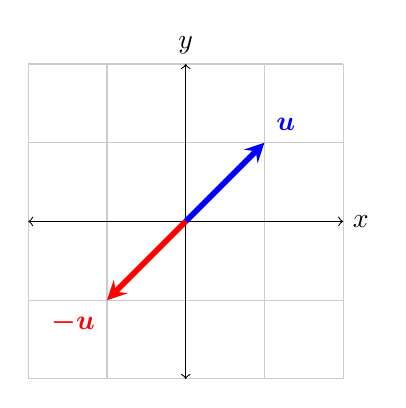
\begin{tikzpicture}
  \draw[thin,gray!40] (-2,-2) grid (2,2);
  \draw[<->] (-2,0)--(2,0) node[right]{$x$};
  \draw[<->] (0,-2)--(0,2) node[above]{$y$};
  \draw[line width=2pt,blue,-stealth](0,0)--(1,1)
        node[anchor=south west]{$\boldsymbol{u}$};
  \draw[line width=2pt,red,-stealth](0,0)--(-1,-1)
        node[anchor=north east]{$\boldsymbol{-u}$};
\end{tikzpicture}
\end{center}
\caption{\label{fig:vectors} Text size inside figure should be as big as
  caption's text. Text size inside figure should be as big as
  caption's text. Text size inside figure should be as big as
  caption's text. Text size inside figure should be as big as
p  caption's text. Text size inside figure should be as big as
  caption's text. }
\end{figure}
%% %---------------------------


Here's a typical reference to a floating figure:
Figure~\ref{fig:vectors}. Floats should usually be placed where latex
wants then. Figure\ref{fig:vectors} is centered, and has a caption
that instructs you to make sure that the size of the text within the
figures that you use is as big as (or bigger than) the size of the
text in the caption of the figures. Please do. Really.

In our case, we've explicitly drawn the figure inlined in latex, to
allow this tex file to cleanly compile. But usually, your figures will
reside in some file.pdf, and you'd include them in your document
with, say, \textbackslash{}includegraphics.

Lists are sometimes quite handy. If you want to itemize things, feel
free:

\begin{description}
  
\item[fread] a function that reads from a \texttt{stream} into the
  array \texttt{ptr} at most \texttt{nobj} objects of size
  \texttt{size}, returning returns the number of objects read.

\item[Fred] a person's name, e.g., there once was a dude named Fred
  who separated usenix.sty from this file to allow for easy
  inclusion.
\end{description}

\noindent
The noindent at the start of this paragraph in its tex version makes
it clear that it's a continuation of the preceding paragraph, as
opposed to a new paragraph in its own right.


\subsection{LaTeX-ing Your TeX File}
%-----------------------------------

People often use \texttt{pdflatex} these days for creating pdf-s from
tex files via the shell. And \texttt{bibtex}, of course. Works for us.

%-------------------------------------------------------------------------------
\section*{Acknowledgments}
%-------------------------------------------------------------------------------

The USENIX latex style is old and very tired, which is why
there's no \textbackslash{}acks command for you to use when
acknowledging. Sorry.

%-------------------------------------------------------------------------------
\section*{Availability}
%-------------------------------------------------------------------------------

USENIX program committees give extra points to submissions that are
backed by artifacts that are publicly available. If you made your code
or data available, it's worth mentioning this fact in a dedicated
section.

%-------------------------------------------------------------------------------
\bibliographystyle{plain}
\bibliography{\jobname}

\end{document}
%%% Local Variables:
%%% mode: latex
%%% TeX-master: t
%%% End:
